\documentclass[tikz,border=3pt]{standalone}
\usepackage{fontspec}
\usepackage{amsmath}
\usepackage{xcolor}
\usepackage{tikz}
\usepackage{pgfplots}
\pgfplotsset{compat=1.18}
\usetikzlibrary{arrows.meta,calc,fit,positioning,shapes.geometric,shapes.misc,patterns,plotmarks}
\IfFontExistsTF{Arial}{\setsansfont{Arial}}{\setsansfont{TeX Gyre Heros}}
\renewcommand{\familydefault}{\sfdefault}
\tikzset{
  >={Stealth[length=2.2mm,width=1.5mm]},
  exact title/.style={font=\bfseries\fontsize{10.5}{12}\selectfont,align=center},
  exact subtitle/.style={font=\fontsize{6.3}{7.2}\selectfont,align=center},
  exact label/.style={font=\fontsize{6.4}{7.5}\selectfont,align=center},
  exact tiny/.style={font=\fontsize{5.3}{6.3}\selectfont,align=center},
  panel/.style={draw=black!14,rounded corners=1.2mm,fill=white,line width=.45pt},
  neutral/.style={draw=black!30,fill=black!3,rounded corners=1mm,line width=.45pt},
  arrow/.style={-Stealth,line width=.7pt},
  softarrow/.style={-Stealth,line width=.55pt,draw=black!45},
  dashedarrow/.style={-Stealth,dashed,line width=.55pt,draw=black!55},
  metric/.style={font=\fontsize{5.3}{6.3}\selectfont,fill=white,inner sep=1pt},
}
\newcommand{\pill}[4]{\node[draw=#2!70,fill=#2!10,rounded corners=1.5mm,inner xsep=3pt,inner ysep=2pt,exact label,text=#2] (#1) at #3 {#4};}
\newcommand{\frameboxx}[4]{\draw[draw=#2!65,fill=#2!8,rounded corners=.6mm,line width=.5pt] (#1.south west) rectangle (#1.north east);\node[exact tiny,text=#2] at #3 {#4};}
\newcommand{\axislabel}[3]{\node[exact tiny,text=black!60] at (#1) {#2};\node[exact tiny,text=black!60,rotate=90] at (#3) {#2};}

\definecolor{dnavy}{HTML}{17324D}\definecolor{dblue}{HTML}{277DA1}\definecolor{dcyan}{HTML}{64C7D8}\definecolor{dyellow}{HTML}{F2C14E}\definecolor{dgreen}{HTML}{55A630}\definecolor{dink}{HTML}{1E293B}
\begin{document}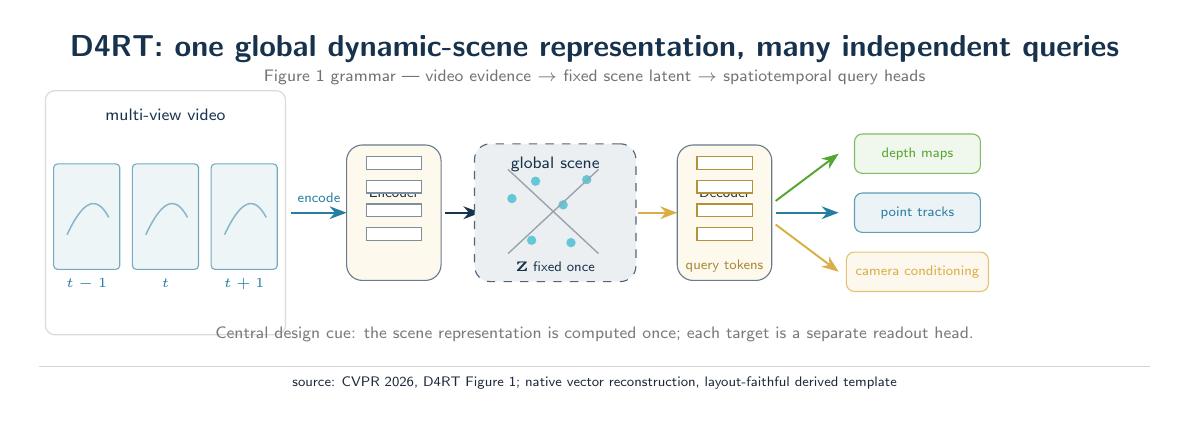
\begin{tikzpicture}[x=1cm,y=1cm]
\path[use as bounding box] (-.2,-2.35) rectangle (14.2,2.35);
\node[exact title,text=dnavy] at (7,2.08) {D4RT: one global dynamic-scene representation, many independent queries};
\node[exact subtitle,text=black!55] at (7,1.72) {Figure 1 grammar — video evidence \(\rightarrow\) fixed scene latent \(\rightarrow\) spatiotemporal query heads};
\node[panel,minimum width=3.05cm,minimum height=3.1cm] (video) at (1.55,0) {};
\node[exact label,text=dnavy] at (1.55,1.25) {multi-view video};
\foreach \x/\t in {0.55/\(t-1\),1.55/\(t\),2.55/\(t+1\)}{
  \draw[draw=dblue!65,fill=dblue!8,rounded corners=.5mm] (\x-.42,-.72) rectangle (\x+.42,.62);
  \draw[dblue!55,line width=.55pt] (\x-.25,-.28) .. controls (\x-.05,.15) and (\x+.12,.24) .. (\x+.28,-.06);
  \node[exact tiny,text=dblue] at (\x,-.9) {\t};
}
\draw[arrow,draw=dblue] (3.15,0) -- (3.85,0) node[midway,above,exact tiny,text=dblue] {encode};
\node[draw=dnavy!65,fill=dyellow!10,rounded corners=2mm,minimum width=1.2cm,minimum height=1.72cm] (enc) at (4.45,0) {};
\node[exact tiny,text=dnavy] at (4.45,.25) {Encoder};\foreach \y in {.55,.25,-.05,-.35}{\draw[dnavy!55,fill=white] (4.1,\y) rectangle (4.8,\y+.16);}
\draw[arrow,draw=dnavy] (5.1,0) -- (5.55,0);
\node[draw=dnavy!75,fill=dnavy!8,rounded corners=2mm,minimum width=2.05cm,minimum height=1.75cm,dashed] (latent) at (6.5,0) {};
\node[exact label,text=dnavy] at (6.5,.62) {global scene};
\foreach \x/\y in {5.95/.18,6.25/.4,6.6/.1,6.9/.42,6.2/-.35,6.7/-.38}{\fill[dcyan] (\x,\y) circle (1.7pt);}\draw[dnavy!45,line width=.5pt] (5.9,-.52)--(7.05,.55);\draw[dnavy!45,line width=.5pt] (5.9,.55)--(7.05,-.52);\node[exact tiny,text=dnavy] at (6.5,-.68) {\(\mathbf{Z}\) fixed once};
\draw[arrow,draw=dyellow!90!black] (7.55,0) -- (8.05,0);
\node[draw=dnavy!65,fill=dyellow!10,rounded corners=2mm,minimum width=1.2cm,minimum height=1.72cm] (dec) at (8.65,0) {};
\node[exact tiny,text=dnavy] at (8.65,.25) {Decoder};\foreach \y in {.55,.25,-.05,-.35}{\draw[dyellow!75!black,fill=white] (8.3,\y) rectangle (9.0,\y+.16);}
\node[exact tiny,text=dyellow!70!black] at (8.65,-.68) {query tokens};
\draw[arrow,draw=dgreen] (9.3,.15) -- (10.1,.75);\draw[arrow,draw=dblue] (9.3,0) -- (10.1,0);\draw[arrow,draw=dyellow!90!black] (9.3,-.15) -- (10.1,-.75);
\foreach \yy/\lab/\c in {.75/depth maps/dgreen,0/point tracks/dblue,-.75/camera conditioning/dyellow!90!black}{\node[draw=\c!75,fill=\c!9,rounded corners=1mm,minimum width=1.6cm,minimum height=.5cm,exact tiny,text=\c] at (11.1,\yy) {\lab};}
\node[exact subtitle,text=black!52] at (7,-1.55) {Central design cue: the scene representation is computed once; each target is a separate readout head.};
\draw[dnavy!20,line width=.45pt] (-.05,-1.95) -- (14.05,-1.95);
\node[exact tiny,text=dink] at (7,-2.16) {source: CVPR 2026, D4RT Figure 1; native vector reconstruction, layout-faithful derived template};
\end{tikzpicture}\end{document}
